\begin{figure}
    \centering
    \begin{subfigure}{0.49\linewidth}
        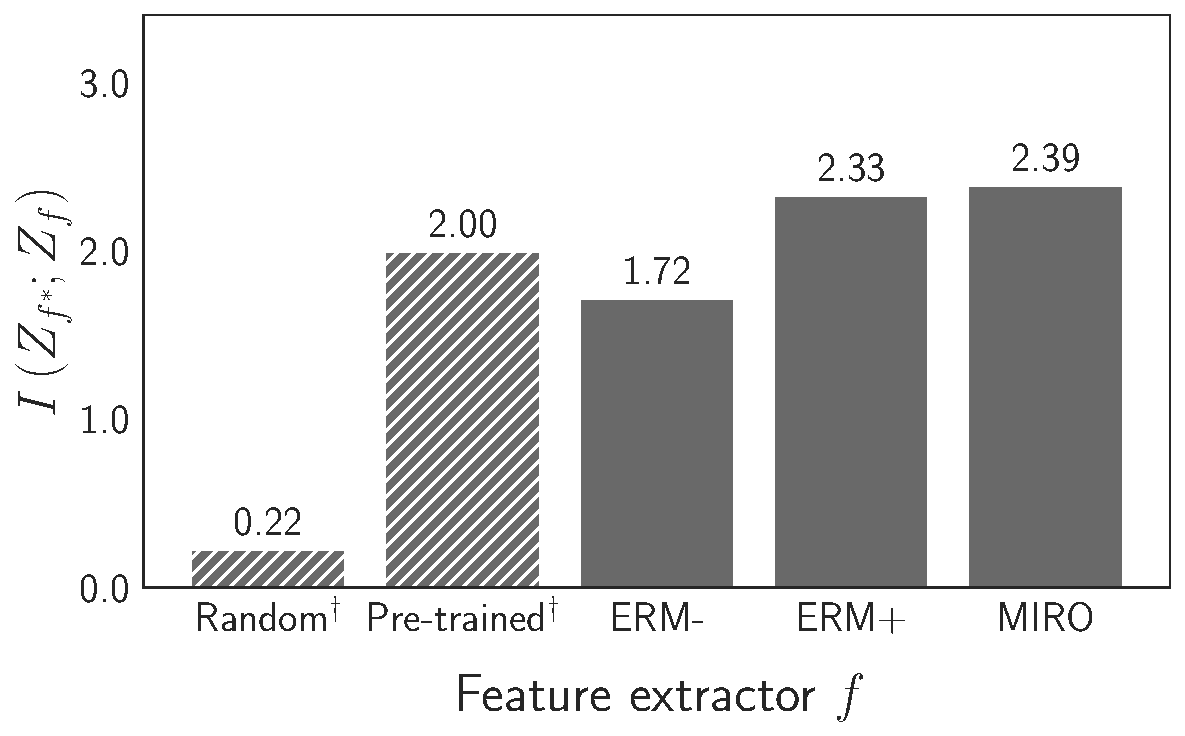
\includegraphics[width=\linewidth]{figures/mi/mi_resnet.pdf}
        \caption{\small ResNet-50}
        \label{fig:mi-resnet}
    \end{subfigure}%
    \hfill
    \begin{subfigure}{0.49\linewidth}
        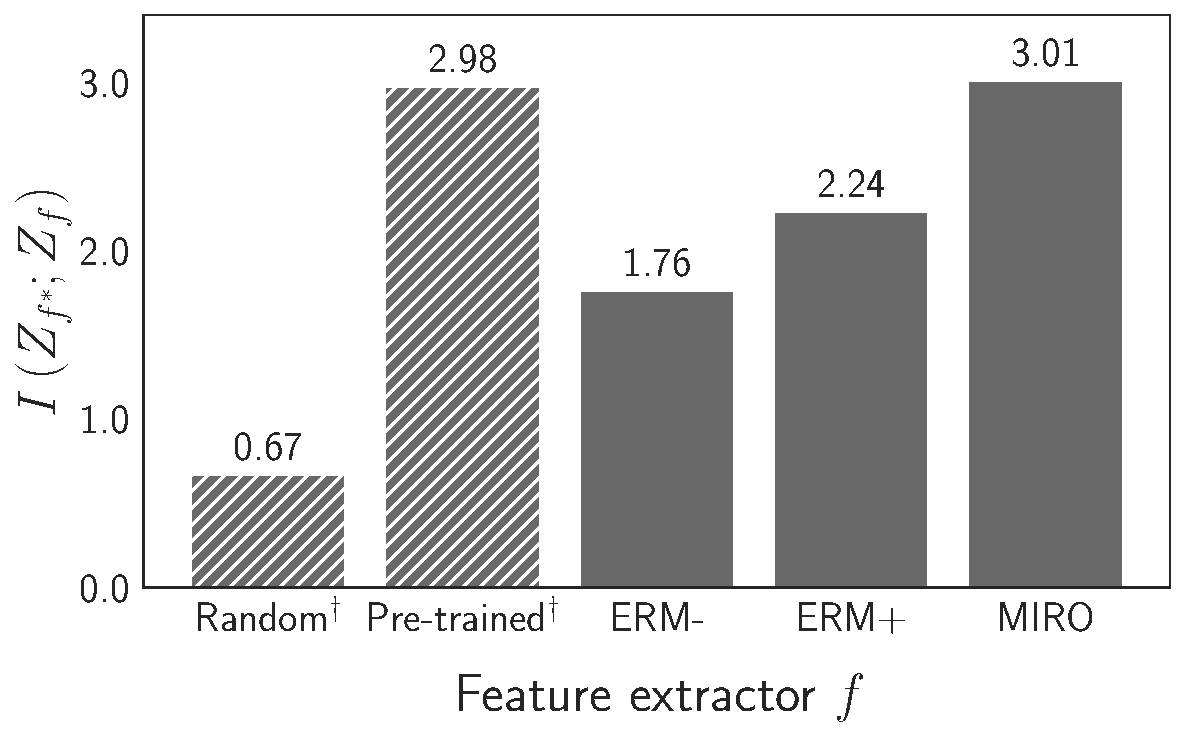
\includegraphics[width=\linewidth]{figures/mi/mi_swag.pdf}
        \caption{\small RegNetY-16GF}
        \label{fig:mi-regnet}
    \end{subfigure}%
    % \begin{subfigure}{0.53\linewidth}
    %     \includegraphics[width=\linewidth]{figures/mi/mi_all.pdf}
    %     \caption{\small All}
    %     \label{fig:mi-all}
    % \end{subfigure}
    \caption{\small \textbf{Mutual information $I\left( Z_{f^{*}}; Z_f \right)$ with oracle model.} The mutual information is estimated by MINE~\cite{belghazi2018mine} in \data{PACS}. Oracle model is trained using all of the four domains. \textit{Random} and \textit{Pre-trained} indicate random and pre-trained model initialization, respectively. \textit{ERM-} and \textit{ERM+} are trained from random and pre-trained model initialization, respectively. $\dagger$ indicates models without fine-tuning. The experiments are repeated with two pre-trained models: ImageNet 1.3M pre-trained ResNet-50 and Instagram 3.6B pre-trained RegNetY-16GF.}
    \label{fig:mi}
    % \vspace{-1em}
\end{figure}



% \begin{figure}
%     \centering
%     \includegraphics[width=0.7\columnwidth]{figures/mi_all.pdf}
%     \caption{\textbf{Mutual information with oracle model.} \textit{Random} is randomly initialized model, \textit{Scratch} is trained by ERM from \textit{Random}, and \textit{Pretrained} is initialized by pretrained model without training. \textit{ERM} and \textit{SIL} is initialized by pretrained model and trained by each method. $\dagger$ indicates RegNetY-16GF pretrained by SWAG is used and ResNet-50 pretrained in ImageNet is used for the others.}
%     \label{fig:mi}
% \end{figure}



